% One-slide teaser for the SFB 1294 Autumn School poster.
% Uses the poster's colors, logos, and declustered Italian catalogue image.
\documentclass[aspectratio=169]{beamer}
\usepackage[T1]{fontenc}
\usepackage{amsmath,amssymb}
\usepackage{graphicx}
\usepackage{xcolor}

\definecolor{upblue}{RGB}{0,48,94}
\definecolor{sfbblue}{RGB}{0,128,181}
\definecolor{postergray}{RGB}{202,204,206}
\setbeamercolor{background canvas}{bg=postergray}
\setbeamercolor{normal text}{fg=black}
\setbeamertemplate{navigation symbols}{}
\setbeamertemplate{footline}{}
\setbeamersize{text margin left=0pt,text margin right=0pt}
\setlength{\fboxsep}{0pt}
\newcommand{\slideequation}[1]{%
  {\color{upblue}\centering\fontsize{16}{19}\selectfont
   $\displaystyle #1$\par}%
}

\begin{document}
\begin{frame}[plain,t]
\noindent\hbox to \paperwidth{%
  \colorbox{upblue}{\parbox[c][1.55cm][c]{3.05cm}{%
    \centering
\includegraphics[width=2.70cm]{sfb_Logo_negativ_Druck.eps}}}%
  \colorbox{sfbblue}{\parbox[c][1.55cm][c]{9.84cm}{%
    \centering\color{white}\sffamily\bfseries\fontsize{15}{18}\selectfont
    Sampling a non-Gaussian\\spatial posterior}}%
  \colorbox{upblue}{\parbox[c][1.55cm][c]{3.05cm}{%
    \centering
\includegraphics[height=1.12cm]{up_logo-weiss.eps}}}%
}\par
\noindent\colorbox{white}{\rule{\paperwidth}{0.05cm}}\par
\vspace{0.18cm}
\noindent\hbox to \paperwidth{%
  \hspace*{0.45cm}%
  \begin{minipage}[t][6.48cm][t]{5.18cm}%
    \vspace*{0pt}\centering
    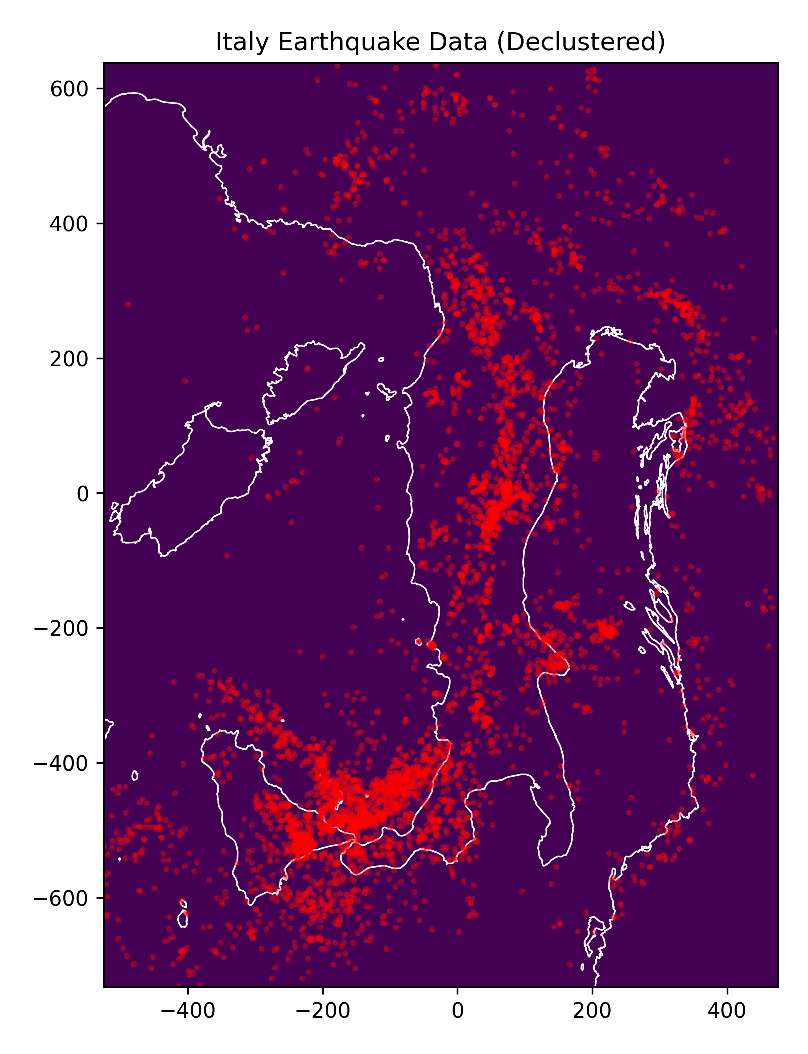
\includegraphics[height=6.20cm]{italy_italy_earthquake_data_bin_5km_declustered.eps}%
  \end{minipage}%
  \hspace*{0.40cm}%
  \begin{minipage}[t][6.48cm][t]{9.42cm}%
  \vspace*{0pt}\colorbox{white}{\parbox[t][6.48cm][t]{9.42cm}{%
    \vspace*{0.10cm}\hspace*{0.27cm}%
    \begin{minipage}[t][6.22cm][t]{8.88cm}
      \colorbox{sfbblue}{\parbox[c][0.54cm][c]{4.25cm}{%
        \centering\color{white}\sffamily\bfseries\fontsize{13}{15}\selectfont
        Gaussian update}}\par
      \vspace{0.10cm}
      {\color{upblue}\sffamily\bfseries\fontsize{10}{12}\selectfont
       Spatial Poisson model\par}
      \vspace{0.03cm}
      \slideequation{n_i\mid f_i\sim\operatorname{Poisson}(\lambda\sigma(f_i))}
      \slideequation{f\sim\mathcal N(\mu,Q^{-1})}
      \vspace{0.08cm}
      {\sffamily\fontsize{10}{12}\selectfont
       Poisson--sigmoid likelihood: non-Gaussian $p(f\mid n)$.\par}
      \vspace{0.10cm}
      \slideequation{Q_{\mathrm{post}}=Q+\operatorname{diag}(\omega)}
      \vspace{0.08cm}
      {\sffamily\fontsize{10}{12}\selectfont
       Poisson and P\'olya--Gamma augmentation makes $f\mid n,k,\omega$
       Gaussian while preserving sparsity.\par}
      \vspace{0.06cm}
      {\color{upblue}\sffamily\bfseries\fontsize{10}{12}\selectfont
       Italy: posterior mean and spatial uncertainty.\par}
      \vfill
      {\color{upblue}\sffamily\fontsize{8}{10}\selectfont
       Toni Luhdo \quad Cristina Ch\'avez Chong \quad Matthias Holschneider\par}
      \vspace{0.12cm}
    \end{minipage}%
  }}%
  \end{minipage}%
  \hfil
}\par
\end{frame}
\end{document}
